\documentclass[handout]{ximera}

\title{Learning Ximera!}
\author{Hilary Freeman}



\begin{document}
\begin{abstract}
  This is a place to get started.
\end{abstract}
\maketitle

I will put some problems here and ask for answers.

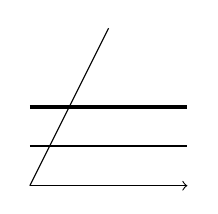
\begin{tikzpicture}
\draw (0,0) --(1,2);
\draw [->] (0,0) -- (2,0);
\draw [ultra thick] (0,1) -- (2,1);
\draw [thick] (0,0.5) -- (2,0.5);
\end{tikzpicture}

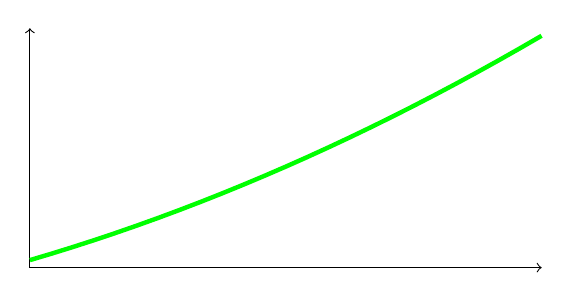
\begin{tikzpicture}[xscale=13,yscale=3.8]
\draw [<->] (0,0.8) -- (0,0) -- (0.5,0);
\draw[green, ultra thick, domain=0:0.5] plot (\x, {0.025+\x+\x*\x});
\end{tikzpicture}

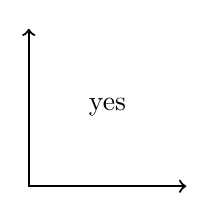
\begin{tikzpicture}
\draw [thick, <->] (0,2) -- (0,0) -- (2,0);
\node at (1,1) {yes};
\end{tikzpicture}

\end{document}
